\documentclass[10pt]{article}
\usepackage{amsmath}
\usepackage{mathtools}
\DeclarePairedDelimiter{\abs}{\lvert}{\rvert}
\usepackage[hidelinks]{hyperref}
\usepackage{amssymb}
\usepackage{tikz}
\usepackage{caption}
\usepackage{graphicx}
\usepackage[T1]{fontenc}
\graphicspath{{.}}
\usepackage{listings}
\usepackage{verbatim}
\usepackage{floatrow}
\usepackage{bigints}
\lstset{
language=[LaTeX]TeX,
backgroundcolor=\color{gray!25},
basicstyle=\ttfamily,
columns=flexible,
breaklines=true
}
\captionsetup{labelsep=colon,justification=centering,singlelinecheck=off}
\reversemarginpar
\usepackage[paper=a4paper,
            %includefoot, % Uncomment to put page number above margin
            marginparwidth=10mm,      % Length of section titles
            marginparsep=0.8mm,       % Space between titles and text
            margin=11mm,              % 25mm margins
            includemp]{geometry}

\begin{document}
\section*{}
\begin{flushleft}
Name: Krishna Chaitanya Sripada\\
\end{flushleft}
\section*{Ans 1}
\begin{flushleft}
Expected adjacency matrix M = $\mathbb{E}$[A] computed over all possible realizations of $\mathcal{B}$ is calculated as follows:\\
\vspace{0.5em}
$\mathbb{E}$[B(p)] = 1 $\times$ p + 0 $\times$ (1 - p) = p and $\mathbb{E}$[B(q)] = 1 $\times$ q + 0 $\times$ (1 - q) = q.\\
\vspace{0.5em}
Given $T$ is a random permutation matrix,\\
\vspace{0.5em}
$$ T = 
\begin{bmatrix} 
1 & \hdots & 0 & 0 & \hdots & 0\\
\vdots & & \vdots & \vdots & & \vdots\\
\vdots & & \vdots & \vdots & & \vdots\\
0 & \hdots & 0 & 1 & \hdots & 0\\
0 & \hdots & 1 & 0 & \hdots & 0\\ 
\vdots & & \vdots & \vdots & & \vdots\\
\vdots & & \vdots & \vdots & & \vdots\\
0 & \hdots & 0 & 0 & \hdots & 1\\
\end{bmatrix}
$$
\vspace{0.5em}
$$ T^{T} = 
\begin{bmatrix} 
1 & \hdots & 0 & 0 & \hdots & 0\\
\vdots & & \vdots & \vdots & & \vdots\\
\vdots & & \vdots & \vdots & & \vdots\\
0 & \hdots & 0 & 1 & \hdots & 0\\
0 & \hdots & 1 & 0 & \hdots & 0\\ 
\vdots & & \vdots & \vdots & & \vdots\\
\vdots & & \vdots & \vdots & & \vdots\\
0 & \hdots & 0 & 0 & \hdots & 1
\end{bmatrix}
$$
Therefore, $A = T\mathcal{B}T^{T} = \mathcal{B}$. By substituting the Bernoulli random variable values, we get, \\
\vspace{0.5em}
$$ M = 
\begin{bmatrix} 
p & \hdots & p & q & \hdots & q\\
\vdots & & \vdots & \vdots & & \vdots\\
\vdots & & \vdots & \vdots & & \vdots\\
p & \hdots & p & q & \hdots & q\\
q & \hdots & q & p & \hdots & p\\ 
\vdots & & \vdots & \vdots & & \vdots\\
\vdots & & \vdots & \vdots & & \vdots\\
q & \hdots & q & p & \hdots & p
\end{bmatrix}
$$
\end{flushleft}
\section*{Ans 2}
\begin{flushleft}
The degree matrix is defined as the diagonal matrix with entries $d_{i} = \sum_{j=1}^{n} A_{i,j} = \frac{1}{2} (n \times p + n \times q) = \frac{n}{2}(p+q)$. Therefore, the expected degree matrix is,\\
\vspace{0.5em}
$$ \mathbb{E}[D] = 
\begin{bmatrix} 
\frac{n}{2}(p+q) & \hdots & 0 & 0 & \hdots & 0\\
\vdots & & \vdots & \vdots & & \vdots\\
\vdots & & \vdots & \vdots & & \vdots\\
0 & \hdots & \frac{n}{2}(p+q) & 0 & \hdots & 0\\
0 & \hdots & 0 & \frac{n}{2}(q+p) & \hdots & 0\\ 
\vdots & & \vdots & \vdots & & \vdots\\
\vdots & & \vdots & \vdots & & \vdots\\
0 & \hdots & 0 & 0 & \hdots & \frac{n}{2}(q+p)
\end{bmatrix}
$$
\end{flushleft}
\section*{Ans 3}
\begin{flushleft}
If $w_{1}$ is an eigenvector of M, then $Mw_{1} = \lambda w_{1}$. Given $w_{1} = \frac{1}{\sqrt n} \mathcal{I}$ where $\mathcal{I}$ =1 $\forall$ i = 1, $\hdots$ , n.\\
\vspace{0.5em}
$$ w_{1} = 
\begin{bmatrix}
\frac{1}{\sqrt n}\\
\vdots\\
\vdots\\
\frac{1}{\sqrt n}\\
\frac{1}{\sqrt n}\\
\vdots\\
\vdots\\
\frac{1}{\sqrt n}
\end{bmatrix}
$$
Then, \\
\vspace{0.5em}
$$ Mw_{1} = 
\begin{bmatrix}
\frac{n}{2 \sqrt n} (p+q)\\
\vdots\\
\vdots\\
\frac{n}{2 \sqrt n} (p+q)\\
\frac{n}{2 \sqrt n} (p+q)\\
\vdots\\
\vdots\\
\frac{n}{2 \sqrt n} (p+q)
\end{bmatrix}
$$
Since $Mw_{1}$ can be expressed as $\lambda w_{1}$, we can say that $w_{1}$ is an eigenvector of M. \\
\vspace{0.5em}
Also the eigenvalue $\mu_{1}$ is given by,\\
\vspace{0.5em}
$$ Mw_{1} = 
\begin{bmatrix}
\frac{n}{2 \sqrt n} (p+q)\\
\vdots\\
\vdots\\
\frac{n}{2 \sqrt n} (p+q)\\
\frac{n}{2 \sqrt n} (p+q)\\
\vdots\\
\vdots\\
\frac{n}{2 \sqrt n} (p+q)
\end{bmatrix}
= \lambda w_{1}
= \begin{bmatrix}
\frac{\lambda}{\sqrt n}\\
\vdots\\
\vdots\\
\frac{\lambda}{\sqrt n}\\
\frac{\lambda}{\sqrt n}\\
\vdots\\
\vdots\\
\frac{\lambda}{\sqrt n}
\end{bmatrix}
$$
Therefore, we have,\\
\vspace{0.5em}
$\frac{n}{2 \sqrt n} (p+q) = \frac{\lambda}{\sqrt n}$\\
\vspace{0.5em}
$\lambda = \frac{n}{2} (p+q)$
\end{flushleft}
\section*{Ans 4}
\begin{flushleft}
To prove that $w_{2}$ is an eigenvector of M. We should be able to prove that $Mw_{2} = \lambda w_{2}$. \\
\vspace{0.5em}
Let $$ w_{2} = 
\begin{bmatrix}
\frac{1}{\sqrt n}\\
\vdots\\
\vdots\\
\frac{1}{\sqrt n}\\
\frac{-1}{\sqrt n}\\
\vdots\\
\vdots\\
\frac{-1}{\sqrt n}
\end{bmatrix}
$$
Then, \\
\vspace{0.5em}
$$ Mw_{2} = 
\begin{bmatrix}
\frac{n}{2 \sqrt n} (p-q)\\
\vdots\\
\vdots\\
\frac{n}{2 \sqrt n} (p-q)\\
\frac{n}{2 \sqrt n} (q-p)\\
\vdots\\
\vdots\\
\frac{n}{2 \sqrt n} (q-p)
\end{bmatrix}
= 
\begin{bmatrix}
\frac{n}{2 \sqrt n} (p-q)\\
\vdots\\
\vdots\\
\frac{n}{2 \sqrt n} (p-q)\\
\frac{-n}{2 \sqrt n} (p-q)\\
\vdots\\
\vdots\\
\frac{-n}{2 \sqrt n} (p-q)
\end{bmatrix}
$$
Since $Mw_{2}$ can be expressed as $\lambda w_{2}$, we can say that $w_{2}$ is an eigenvector of M. \\
\vspace{0.5em}
Also the eigenvalue $\mu_{2}$ is given by,\\
\vspace{0.5em}
$$ Mw_{2} = 
\begin{bmatrix}
\frac{n}{2 \sqrt n} (p-q)\\
\vdots\\
\vdots\\
\frac{n}{2 \sqrt n} (p-q)\\
\frac{-n}{2 \sqrt n} (p-q)\\
\vdots\\
\vdots\\
\frac{-n}{2 \sqrt n} (p-q)
\end{bmatrix}
= \lambda w_{2}
= \begin{bmatrix}
\frac{\lambda}{\sqrt n}\\
\vdots\\
\vdots\\
\frac{\lambda}{\sqrt n}\\
\frac{-\lambda}{\sqrt n}\\
\vdots\\
\vdots\\
\frac{-\lambda}{\sqrt n}
\end{bmatrix}
$$
Therefore, we have,\\
\vspace{0.5em}
$\frac{n}{2 \sqrt n} (p-q) = \frac{\lambda}{\sqrt n}$\\
\vspace{0.5em}
$\lambda = \frac{n}{2} (p-q)$
\end{flushleft}
\section*{Ans 5}
\begin{figure}[!htb]
    \begin{floatrow}
         \ffigbox{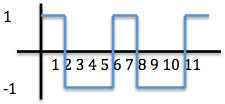
\includegraphics[scale = 0.8]{w3.png}}{\caption{Graph of $w_{3}$}\label{w3}}
         \ffigbox{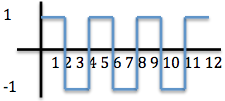
\includegraphics[scale = 0.8]{w4.png}}{\caption{Graph of $w_{4}$}\label{w4}}
    \end{floatrow}
\end{figure}
\section*{Ans 6}
\begin{flushleft}

\end{flushleft}
\end{document}